%%%%%%%%%%%%%%%%%%%%%%%%%%%%%%%%%%%%%%%%%%%%%%%%%%%
%% LaTeX book template                           %%
%% Author:  Amber Jain (http://amberj.devio.us/) %%
%% License: ISC license                          %%
%%%%%%%%%%%%%%%%%%%%%%%%%%%%%%%%%%%%%%%%%%%%%%%%%%%

\documentclass[a4paper,11pt]{book}
\usepackage[T1]{fontenc}
\usepackage[utf8]{inputenc}
\usepackage{lmodern}
%%%%%%%%%%%%%%%%%%%%%%%%%%%%%%%%%%%%%%%%%%%%%%%%%%%%%%%%%
% Source: http://en.wikibooks.org/wiki/LaTeX/Hyperlinks %
%%%%%%%%%%%%%%%%%%%%%%%%%%%%%%%%%%%%%%%%%%%%%%%%%%%%%%%%%
\usepackage{hyperref}
\usepackage{graphicx}
\usepackage[english]{babel}

\usepackage{lscape}
\usepackage{caption}
\captionsetup{tableposition=top,figureposition=bottom,font=small}
%%%%%%%%%%%%%%%%%%%%%%%%%%%%%%%%%%%%%%%%%%%%%%%%%%%%%%%%%%%%%%%%%%%%%%%%%%%%%%%%
% 'dedication' environment: To add a dedication paragraph at the start of book %
% Source: http://www.tug.org/pipermail/texhax/2010-June/015184.html            %
%%%%%%%%%%%%%%%%%%%%%%%%%%%%%%%%%%%%%%%%%%%%%%%%%%%%%%%%%%%%%%%%%%%%%%%%%%%%%%%%
\newenvironment{dedication}
{
   \cleardoublepage
   \thispagestyle{empty}
   \vspace*{\stretch{1}}
   \hfill\begin{minipage}[t]{0.66\textwidth}
   \raggedright
}
{
   \end{minipage}
   \vspace*{\stretch{3}}
   \clearpage
}

%%%%%%%%%%%%%%%%%%%%%%%%%%%%%%%%%%%%%%%%%%%%%%%%
% Chapter quote at the start of chapter        %
% Source: http://tex.stackexchange.com/a/53380 %
%%%%%%%%%%%%%%%%%%%%%%%%%%%%%%%%%%%%%%%%%%%%%%%%
\makeatletter
\renewcommand{\@chapapp}{}% Not necessary...
\newenvironment{chapquote}[2][2em]
  {\setlength{\@tempdima}{#1}%
   \def\chapquote@author{#2}%
   \parshape 1 \@tempdima \dimexpr\textwidth-2\@tempdima\relax%
   \itshape}
  {\par\normalfont\hfill--\ \chapquote@author\hspace*{\@tempdima}\par\bigskip}
\makeatother

%%%%%%%%%%%%%%%%%%%%%%%%%%%%%%%%%%%%%%%%%%%%%%%%%%%
% First page of book which contains 'stuff' like: %
%  - Book title, subtitle                         %
%  - Book author name                             %
%%%%%%%%%%%%%%%%%%%%%%%%%%%%%%%%%%%%%%%%%%%%%%%%%%%

% Book's title and subtitle
\title{\Huge \textbf{Gestione di un sistema di book-crossing} \\ \huge \textit{\textbf{Documentazione progettuale}} \\ \bigskip \huge Progetto del corso di Informatica IIIB \\ \huge A.A. 2018/2019}
% Author
\author{\textsc{Paganessi Andrea} \\ \textsc{Piffari Michele} \\ \textsc{Villa Stefano}}


\begin{document}

\frontmatter
\maketitle

%%%%%%%%%%%%%%%%%%%%%%%%%%%%%%%%%%%%%%%%%%%%%%%%%%%%%%%%%%%%%%%%%%%%%%%%
% Auto-generated table of contents, list of figures and list of tables %
%%%%%%%%%%%%%%%%%%%%%%%%%%%%%%%%%%%%%%%%%%%%%%%%%%%%%%%%%%%%%%%%%%%%%%%%
\tableofcontents
\listoffigures
\listoftables

\mainmatter

%%%%%%%%%%%%%%%%
% NEW PART! %
%%%%%%%%%%%%%%%%
\part{Iterazione 0}

%%%%%%%%%%%%%%%%
% NEW CHAPTER! %
%%%%%%%%%%%%%%%%
\chapter{Requisiti e specifiche}
\section{Requisiti utente}
La startUp bergamasca Book Crossing UniBg desidera mettere a disposizione dei propri
utenti un'applicazione Android per poter gestire la libera condivisione di libri all'interno di una vasta community di utenti.

I libri della rete di BookCrossing che l'azienda punta a gestire si possono trovare
\begin{itemize}
	\item Casualmente (in stazione, su una panchina, in un locale o in un qualsiasi altro luogo): funzionalità \textit{"on the go"}
	\item Nella zona di scambio ufficiale (\textit{"OCZ UniBg"}: Official Crossing Zone UniBg)
\end{itemize}

Per il momento, l'unica OCZ gestita direttamente dalla startUp si trova all'interno dell'aula studio del campus di Ingegneria di Dalmine, la quale coincide anche con la sistemazione del server centrale che andrà a gestire i vari interscambi tra gli users.

La startUp richiede che, per usufruire dell'applicativo mobile, i clienti debbano registrarsi fornendo i propri dati quali
\begin{itemize}
	\item Nome
	\item Cognome
	\item Contatto di riferimento (opzionale)
	\begin{itemize}
		\item Numero telefonico
		\item Indirizzo mail
		\item Facebook
		\item ID Twitter
	\end{itemize}
	\item Categorie di libri preferite
	\item Zona di residenza
\end{itemize}

Una volta registratosi, l'utente può partecipare al programma di Book Crossing.

Secondo la politica del book sharing, per rendere disponibile alla comunità 
uno o più libri che non sono ancora presenti nel network stesso, 
serve
identificarli univocamente, per poterne così tracciare la storia, ovvero ciò 
che concerne il percorso seguito dal libro, le recensioni lasciate dagli utenti etc.

Prima di procedere con l'identificazione univoca del libro, l'utilizzatore deve inserire i dati 
del testo (o dei testi) che intende condividere con il resto della community: questo inserimento può avvenire
- In maniera "automatica" tramite scansione del codice ISBN
- In modalità "manuale", nel caso in cui, per esempio, non sia presente il barcode, fornendo i 
seguenti dati:
\begin{itemize}
	\item Titolo
	\item Autore
	\item Anno di pubblicazione/Edizione
	\item Categoria
\end{itemize}

A questo punto il sistema genererà un BCID di 10 caratteri, ovvero un \textit{Book Crossing ID} univoco, il
quale dovrà essere riportato sul testo dall'utente.


La vera e propria condivisione avviene nel momento in cui il volume/i viene rilasciato (azione che può avvenire in un secondo momento
rispetto alla fase di identificazione), il sistema dovrà acquisire i seguenti dati:
\begin{itemize}
	\item Luogo di rilascio (con estensione future per un'acquisizione automatica della posizione tramite GPS)
	\item Ora e data di rilascio 
\end{itemize}

L'app inoltre consiglierà all'utente un luogo di rilascio in cui sia già presente almeno un libro, 
facilitando così la creazione di cassette virtuali, ovvero di luoghi in cui sono presenti più libri: 
l'idea è quella quindi di permettere al sistema di creare, in maniera autonoma, dei punti "fissi" di 
consegna senza dover applicare interventi a livello infrastrutturale.

Successivamente il sistema dovrà notificare gli utenti, interessati al genere del 
libro rilasciato, della presenza di un nuovo testo, appena rilasciato, che potrebbe interessargli.

In qualsiasi momento è possibile effettuare le seguenti operezioni su ogni libro personalmente 
condiviso con la rete di sharing:
\begin{itemize}
	\item Aggiunta di recensione
	\item Rating del libro
\end{itemize}

Quando viene trovato un libro (nel gergo definito come \textit{"journal entry"}), il cliente che vuole prelevarlo, dopo
aver effettuato il login nell'applicazione, deve inserire nell'apposito menù il BCID del libro che intende acquisire.
Il sistema si occuperà poi di informare la community aggiornando lo status del libro raccolto, che diventerà "underReading".

Per quanto concerne invece l'area riservata, ogni utente ha la possibilità di 
visualizzare informazioni in merito ai libri che: 
\begin{itemize}
	\item ha messo a disposizione della community (\textbf{relased})
	\item ha ottenuto dalla community (\textbf{chased})
	\item attualmente possiede
\end{itemize}

L'utente può effettuare la prenotazione di libri già inseriti nella liste "chased" e "relased" del proprio profilo.


Il sistema deve prevedere anche la possibilità di ricercare un specifico testo e visualizzare i contatti dei
lettori del libro al fine di potersi scambiare opinioni e/o pareri in merito al libro stesso.
Tale funzionalità di ricerca permette anche la prenotazione del testo ricercato purché lo stesso sia nello
stato "under reading".
Per soddisfare questa richiesta il sistema provvederà a consigliare, al lettore corrente 
del libro prenotato, zone di rilascio specifiche al fine di avvicinare tale libro al richiedente, tenendo presente anche la necessità di creare cassette virtuali (come specificato in precedenza).
\chapter{Use cases}
\section{Analisi testuale dei casi d'uso}


\begin{itemize}
	\item \textbf{\textit{UC1: Registration}}
	\begin{itemize}
		\item \textbf{Descrizione:} registrazione alla rete di Book Crossing.
		\item \textbf{Attori coinvolti:} utente.
		\item \textbf{Preconditions:} 
		\begin{itemize}
			\item smartphone dotato di connessione dati;
			\item l’utente non è ancora registrato al programma di Book Crossing.
		\end{itemize}
		\item \textbf{Postconditions:} l’utente è registrato al programma di Book Crossing.
		\item \textbf{Processo:}
		\begin{enumerate}
			\item l’utente seleziona “Registrati” nella schermata inziale dell’applicazione;
			\item l’applicazione mostra un form in cui l'utente può inserire:
			\begin{enumerate}
				\item [a.] Nome
				\item [b.] Cognome
				\item [c.] Data di nascita
				\item [d.] Username
				\item [e.] Password
				\item [f.] Contatto di riferimento
				\item [g.] Categorie di libri preferite
				\item [h.] Zona di residenza
				\item [i.] Raggio d'azione rispetto alla zona di residenza
			\end{enumerate}
			\item l’utente inserisce i dati richiesti nel form presentato;
			\item l'utente attende la visualizzazione della conferma di avvenuta registrazione;
			\item l’utente viene reindirizzato alla pagina principale dell’applicazione.
		\end{enumerate}
		\item \textbf{Alternative}
		\begin{itemize}
			\item \textbf{Dati non validi:} se l'utente inserisce dei dati non validi e/o mancanti, l'applicazione mostra un messaggio d'errore permettendo all'utente di modificare i dati non validi.
		\end{itemize}
		\item \textbf{Estensioni}
	\end{itemize}
	\item \textbf{\textit{UC2: Login}}
	\begin{itemize}
		\item \textbf{Descrizione:} accesso alla rete di Book Crossing.
		\item \textbf{Attori coinvolti:} utente. 
		\item \textbf{Preconditions:} 
		\begin{itemize}
			\item smartphone dotato di connessione dati;
			\item l’utente è già registrato al programma di Book Crossing.
		\end{itemize}
		\item \textbf{Postconditions:} l’utente è loggato nella rete di Book Crossing.
		\item \textbf{Processo:}
		\begin{enumerate}
			\item l’utente seleziona “Login” nella schermata iniziale dell’applicazione;
			\item l’applicazione mostra una schermata in cui l'utente inserisce username e password;
			\item l’utente inserisce i dati richiesti nella view presentata;
			\item l'utente attende la verifica della correttezza dei dati inseriti;
			\item l’utente viene reindirizzato alla pagina principale dell’applicazione.
		\end{enumerate}
		\item \textbf{Alternative}
		\begin{itemize}
			\item \textbf{Username e/o password non corretti:}  se l'utente inserisce username e/o password non validi, l'applicazione mostra un messaggio d'errore permettendo all'utente di modificare i dati.
		\end{itemize}
		\item \textbf{Estensioni}
	\end{itemize}
		\item \textbf{\textit{UC3: Logout}}
	\begin{itemize}
		\item \textbf{Descrizione:} disconnessione profilo personale.
		\item \textbf{Attori coinvolti:} utente. 
		\item \textbf{Preconditions:} 
		\begin{itemize}
			\item smartphone dotato di connessione dati;
			\item l’utente è già registrato al programma di Book Crossing;
			\item l'utente è loggato.
		\end{itemize}
		\item \textbf{Postconditions:} l’utente non è più loggato nella rete di Book Crossing.
		\item \textbf{Processo:}
		\begin{enumerate}
			\item l’utente seleziona “Profilo personale” nella schermata principale dell’applicazione;
			\item l’applicazione mostra una schermata in cui l'utente può visualizzare tutte le proprie informazioni;
			\item l’utente preme il bottone "Logout";
			\item l’utente viene reindirizzato alla pagina di login.
		\end{enumerate}
	\end{itemize}

	\item \textit{\textbf{UC4: Book pick-up}}
	\begin{itemize}
		\item \textbf{Descrizione:} raccolta di un libro “on the go”\footnote{In questo caso il libro condiviso dalla community viene raccolto dall'utente in una qualsiasi zona (come per esempio la stazione, il parco, sale di attesa etc...).} o in una OCZ.\footnote{\textit{Official Crossing Zone}: zone riconosciute e fisse in cui la community può liberamente scambiarsi i libri.}
		\item \textbf{Attori coinvolti:} utente.
		\item \textbf{Preconditions:}
		\begin{itemize}
			\item smartphone dotato di connessione dati;
			\item l’utente ha effettuato l’accesso alla rete di Book Crossing;
			\item il libro è stato siglato con il codice BCID.
		\end{itemize}
		\item \textbf{Postconditions:} Il libro viene associato all’utente.
		\item \textbf{Processo:}
		\begin{enumerate}
			\item l’utente seleziona “Raccogli libro” nel menu principale dell’applicazione;
			\item l’applicazione mostra un form in cui l’utente può inserire il BCID del libro;
			\item l’utente inserisce il codice BCID riportato nel libro;
			\item l'utente attende la visualizzazione di una scheda riepilogativa relativa al libro appena aggiunto;
			\item l’utente verifica la corrispondenza delle informazioni mostrate;
			\item l'utente conferma la raccolta.
		\end{enumerate}
		\item \textbf{Alternative}
		\begin{itemize}
			\item \textbf{BCID inesistente:} se l'utente inserisce un BCID non esistente, l'applicazione mostra un messaggio d'errore permettendo all'utente di modificare il BCID.
			\item \textbf{BCID associato ad un altro utente:} se l'utente inserisce un BCID già in possesso di un'altro utente, l'applicazione mostra un messaggio d'errore permettendo all'utente di modificare il BCID.
			\item \textbf{BCID non corrispondente:} se l'utente, al punto (4), verifica che il libro reale non corrisponde alle informazioni mostrate dall'applicazione, può annullare l'operazione di raccolta.
		\end{itemize}
		\item \textbf{Estensioni}
	\end{itemize}
	\item \textbf{\textit{UC5: Book registration}}
	\begin{itemize}
		\item \textbf{Descrizione:} registrazione di un libro alla rete di Book Crossing (\textit{journal entry}).
		\item \textbf{Generalizzazione di:} 
		\begin{itemize}
			\item aggiunta manuale dei dati del libro (UC8);
			\item scansione ISBN (UC9).
		\end{itemize}
		\item \textbf{Include:} scrittura BCID (UC10).
		\item \textbf{Attori coinvolti:} utente.
		\item \textbf{Preconditions:}
		\begin{itemize}
			\item smartphone dotato di connessione dati;
			\item l’utente ha effettuato l’accesso alla rete di Book Crossing;
			\item il libro non è ancora stato siglato con il codice BCID.
		\end{itemize}
		\item \textbf{Postconditions:} Il libro viene registrato alla rete di Book Crossing.		
		\item \textbf{Processo:} 
		\begin{enumerate}
			\item l’utente seleziona “Registra un nuovo libro” nel menu principale dell’applicazione;
			\item l’applicazione tenta di iniziare la scansione ISBN mostrando all'utente la fotocamera;
			\item l’utente inquadra il codice ISBN del libro per il tempo sufficiente al riconoscimento del codice stesso;
			\item l’applicazione mostra all'utente la schermata contente tutti le informazioni del libro; 
			\item l'utente preme il pulsante "Conferma registrazione", dopo aver verficato rapidamente la coerenza dei dati.
		\end{enumerate}
		\item \textbf{Alternative}
		\begin{itemize}
			\item \textbf{Aggiunta manuale dei dati:} se, dalla schermata di scansione, l'utente decide di inserire manualmente i dati del libro da registrate, l'applicazione mostra una schermata dove aggiungere manualmente i dati del libro.
			\item \textbf{Scansione fallita:} se la scansione fallisce, l'applicazione riapre la fotocamenra permettendo all'utente di ripetere l'operazione.
		\end{itemize}
		\item \textbf{Estensioni}
	\end{itemize}
	\item \textbf{\textit{UC6: Book research}}
	\begin{itemize}
		\item \textbf{Descrizione:} ricerca di un libro all’interno della rete di Book Crossing.
		\item \textbf{Attori coinvolti:} utente.
		\item \textbf{Preconditions:}
		\begin{itemize}
			\item smartphone dotato di connessione dati;
			\item l’utente ha effettuato l’accesso alla rete di Book Crossing;
			\item il libro è presente nella rete di Book Crossing.
		\end{itemize}
		\item \textbf{Postconditions:} il libro ricercato viene mostrato.
		\item \textbf{Processo:}
		\begin{enumerate}
			\item l’utente seleziona “Ricerca libro” nel menu principale dell’applicazione;
			\item l’applicazione mostra all'utente un form da completare in cui inserire i parametri della ricerca;
			\item l’utente inserisce i parametri a cui è interessato;
			\item l'utente preme il pulsante "Cerca" ed attende il completamento;
			\item l'utente visualizza la lista di tutti i libri nella rete, che soddisfano la ricerca.
			\item il sistema verifica la presenza del libro cercato;
			\item in caso di esito positivo, l’applicazione mostra una scheda riassuntiva del libro;
			\item in caso di esito negativo, l’applicazione mostrerà un messaggio di errore;
		\end{enumerate}
		\item \textbf{Alternative}
		\begin{itemize}
			\item \textbf{Parametri non validi:}se l'utente inserisce dei parametri non validi, l'applicazione mostra un messaggio d'errore permettendo all'utente di modificarli.
			\item \textbf{Ricerca senza risultati:} se la ricerca non va a buon fine, l'applicazione mostra un messaggio all'utente, comunicando che nessun libro presente nella rete soddisfa i parametri di ricerca inseriti.
		\end{itemize}
		\item \textbf{Estensioni}
		\begin{itemize}
			\item L'utente può selezionare uno dei libri mostrati dall'applicazione e visualizzare le sue informazioni.
		\end{itemize}
	\end{itemize}
	\item \textbf{\textit{UC7: Info visualization}}
	\begin{itemize}
		\item \textbf{Descrizione: } Visualizzazione informazioni
		\item \textbf{Generalizzazione:} visualizzazione informazioni libri chased(UC13), visualizzazione informazioni libri relased(UC14), visualizzazione informazioni libri in possesso(UC15)
		\item \textbf{Attori coinvolti:} Utente
		\item \textbf{Preconditions:}
		\begin{itemize}
			\item smartphone dotato di connessione dati;
			\item l’utente ha effettuato l’accesso alla rete di Book Crossing;
		\end{itemize}
		\item \textbf{Postconditions:} L’applicazione mostra le informazioni desiderate
		\item \textbf{Processo:}
		\begin{enumerate}
			\item l’utente seleziona la voce “I miei libri” nel menu principale dell’applicazione;
			\item l’applicazione mostra categorie di informazioni visualizzabili;
			\item l’utente seleziona la categoria che vuole visualizzare;
			\item l'applicazione mostro l'elenco dei libri della categoria selezionata.
		\end{enumerate}
		\item \textbf{Alternative}
		\begin{itemize}
			\item \textbf{Nessun libro in elenco:}se nessun libro è presente nello storico, l'applicazione mostra un messaggio all'utente, comunicando che non è stata ancora effettuata nessuna operazione nella comunità.
		\end{itemize}
		\item \textbf{Estensioni}
	\end{itemize}
	\item \textbf{\textit{UC8: Personal area visualization}}
	\begin{itemize}
		\item \textbf{Descrizione: } Visualizzazione profilo personale utente
		\item \textbf{Attori coinvolti:} Utente
		\item \textbf{Preconditions:}
		\begin{itemize}
			\item smartphone dotato di connessione dati;
			\item l’utente ha effettuato l’accesso alla rete di Book Crossing;
		\end{itemize}
		\item \textbf{Postconditions: }L’applicazione mostra il profilo dell’utente.
		\item \textbf{Processo: }
		\begin{enumerate}
			\item l’utente seleziona la voce “Il mio profilo” nel menu principale dell’applicazione;
			\item l’applicazione mostra l’anagrafica, i contatti e le attività svolte dall’utente;
		\end{enumerate}
		\item \textbf{Estensioni:}
	\end{itemize}
	\item \textbf{\textit{UC9: Manual addition of book's data}}
	\begin{itemize}
		\item \textbf{Descrizione:} Inserimento manuale di un libro nella rete di Book Crossing
		\item \textbf{Attori coinvolti:} Utente
		\item \textbf{Preconditions:}
		\begin{itemize}
			\item smartphone dotato di connessione dati;
			\item l’utente ha effettuato l’accesso alla rete di Book Crossing;
			\item il libro non è stato ancora siglato con il codice BCID;
		\end{itemize}
		\item \textbf{Postcondition:} Viene generato il codice BCID e il libro viene aggiunto alla rete di Book Crossing
		\item \textbf{Processo: }
		\begin{enumerate}
			\item facendo riferimento al passo 1 e 2 del UC4, l'utente preme il pulsante “Aggiunta manuale”;
			\item l’applicazione mostra un form da compilare con i dati del libro;
			\item l’utente inserisce i dati del libro richiesti e conferma l’operazione;
			\item l’applicazione mostra il codice BCID da trascrivere sul libro;
			\item il sistema aggiunge il libro alla rete di Book Crossing;
		\end{enumerate}
		\item \textbf{Estensioni}
	\end{itemize}
	\item \textbf{\textit{UC10: ISBN scan}}
	\begin{itemize}
		\item \textbf{Descrizione:} scansione del codice ISBN tramite fotocamera per ottenere le informazioni in merito al libro da registrare.
		\item \textbf{Attori coinvolti:} utente
		\item {Preconditions:} 
		\begin{itemize}
			\item smartphone dotato di connessione dati;
			\item l’utente ha effettuato l’accesso alla rete di Book Crossing;
			\item il libro possiede il codice ISBN.
		\end{itemize}
		\item \textbf{Postconditions:} il libro è in possesso dell'utente e non più condiviso con la community.
		\item \textbf{Processo:}
		\begin{enumerate}
			\item l’utente seleziona “Registra un nuovo libro” nel menu principale dell’applicazione;;
			\item Viene aperta la fotocamera all'interno dell'applicazione;
			\item l'utente inquadra il codice ISBN finchè il sistema non rileva il barcode.
		\end{enumerate}
		\item \textbf{Alternative}
		\begin{itemize}
			\item \textbf{ISBN non riconsciuto:} il sistema non è in grado di riconoscere l'ISBN inquadrato. Si chiuderà la fotocamera e l'utente verrà reindirizzato alla pagina di inserimento manuale del libro(UC9).
		\end{itemize}
		\item \textbf{Estensioni}
	\end{itemize}
	\item \textbf{\textit{UC11: Instruction to write BCID code\footnote{\textit{Book Crossing IDentifier}}}}
	\begin{itemize}
		\item \textbf{Descrizione:} scrittura del codice identificativo sul libro condiviso.
		\item \textbf{Attori coinvolti:} utente
		\item \textbf{Preconditions:}
		\begin{itemize}
			\item smartphone dotato di connessione dati;
			\item l’utente ha effettuato l’accesso alla rete di Book Crossing;
		\end{itemize}
		\item \textbf{Postconditions:} il libro è univocamente riconosciuto del sistema tramite il BCID.
		\item \textbf{Processo:} l'utente copia il codice BCID sul libro, seguendo le istruzioni mostrate dall'applicazione.
		\item \textbf{Estensioni}
	\end{itemize}
	\item \textbf{\textit{UC12: View of users contacts}}
	\begin{itemize}
		\item \textbf{Descrizione:} l'utente ottiene i contatti che un altro utilizzatore ha deciso di condividere con la community.
		\item \textbf{Attori coinvolti:} utente
		\item \textbf{Preconditions:}
		\begin{itemize}
			\item smartphone dotato di connessione dati;
			\item l’utente ha effettuato l’accesso alla rete di Book Crossing.
		\end{itemize}
		\item \textbf{Postconditions:} l'applicazione visualizza i contatti a cui l'utente può e/o vuole essere contattato.
		\item \textbf{Processo:}
		\begin{enumerate}
			\item l'utente selezione "Ricerca" dal menu principale dell'applicazione;
			\item l'utente seleziona il libro a cui è interessato;
			\item il sistema mostra tutte le informazioni relative al libro (tra cui anche la lista di tutti i lettori che sono stati in possesso del libro in questione);
			\item l'utlizzatore seleziona l'utente che desidera contattare;
			\item il sistema mostra tutte le informazioni di contatto che il cliente terzo ha deciso di condividere con la community.
		\end{enumerate}
		\item \textbf{Alternative:}
		\begin{itemize}
			\item \textbf{Nessun libro trovato:} la grafica notifica l'utilizzatore del fatto che la ricerca non sia andata a buon fine.
			\item \textbf{Utente senza alcun contatto condiviso:} il sistema filtra la visualizzazione della lista degli utenti, visualizzando solo coloro che hanno inserito, durante la fase di registrazione, almeno un contatto o che desiderano essere contattati.
		\end{itemize}
		\item \textbf{Estensioni}
	\end{itemize}
	\item \textbf{\textit{UC13: Book reservation}}
	\begin{itemize}
		\item \textbf{Descrizione:} l'utilizzatore prenota un determinato libro in possesso di un altro lettore.
		\item \textbf{Attori coinvolti:}
		\begin{itemize}
			\item utente richiedente \textit{claimant user};
			\item utente attualmente in possesso del libro richiesto \textit{owner user}.
		\end{itemize}
		\item \textbf{Preconditions:}
		\begin{itemize}
			\item smartphone dotato di connessione dati;
			\item l’utente ha effettuato l’accesso alla rete di Book Crossing;
			\item il libro che si vuole prenotare deve essere registrato alla rete;
			\item il libro richiesto deve essere già in possesso di un altro utente;
		\end{itemize}
		\item \textbf{Postconditions:}
		\begin{itemize}
			\item Se i due utenti hanno un punto di incontro in comune, si accordano sul luogo di scambio. 
			\item Se, invece, non hanno un punto di incontro comune, il libro passerà tra gli utenti che si trovano tra \textit{claimant user} e \textit{owner user}.
		\end{itemize}
		\item \textbf{Processo:}
		\begin{enumerate}
			\item l’utente seleziona “Ricerca libro” nel menu principale dell’applicazione;
			\item l’applicazione mostra all'utente un form da completare in cui inserire i parametri della ricerca;
			\item l’utente inserisce i parametri a cui è interessato;
			\item l'utente preme il pulsante "Cerca" ed attende il completamento;
			\item l'utente visualizza la lista di tutti i libri nella rete, che soddisfano la ricerca.
			\item il sistema verifica la presenza del libro cercato;
			\item l'utente va a selezionare il libro all'interno della lista proposta dal sistema;
			\item l'applicazione mostra un riepilogo sulle informazioni del libro, unitamente alla possibilità di prenotare;
			\item l'utente preme il pulsante "Prenota";
			\item l'applicazione mostra una pagina di conferma dell'avvenuta prenotazione.
		\end{enumerate}
		\item \textbf{Alternative}
		\begin{itemize}
			\item \textbf{Libro non prenotabile:} il libro selezionato non è prenotabile poichè non in possesso di un altro utente.
		\end{itemize}
		\item \textbf{Estensioni}
	\end{itemize}
	\item \textbf{\textit{UC13: Visualizzazione info libri chased}}
	\begin{itemize}
		\item \textbf{Descrizione:} visualizzazione storico dei libri "raccolti" dall'utente.
		\item \textbf{Attori coinvolti:} utente finale.
		\item \textbf{Preconditions:}
		\begin{itemize}
			\item smartphone dotato di connessione dati;
			\item l’utente ha effettuato l’accesso alla rete di Book Crossing.
		\end{itemize}
		\item \textbf{Postconditions:} mostrata sulla grafica la lista dei libri raccolti, con relativa data e luogo di "chasing".
		\item \textbf{Processo:}
		\begin{enumerate}
			\item l'utente, dal menù principale dell'applicazione, entra nella propria area riservata;
			\item l'applicazione mostrerà un riassunto delle informazioni dell'utilizzatore;
			\item l'utente va preme il pulsante "Libri chased";
			\item l'applicazione mostra un riepilogo di tutti i testi ottenuti dalla community di sharing.
		\end{enumerate}
		\item \textbf{Alternative:}
		\begin{itemize}
			\item \textbf{Nessun libro chased:} la grafica notifica l'utilizzatore del fatto che non sia ancora stata effettuata una raccolta di almeno un volume.
		\end{itemize}
		\item \textbf{Estensioni}
	\end{itemize}
	\item \textbf{\textit{UC14: Visualizzazione info libri released}}
	\begin{itemize}
		\item \textbf{Descrizione:} visualizzazione storico dei propri libri condivisi con la rete.
		\item \textbf{Attori coinvolti:}  utente finale.
		\item \textbf{Preconditions:}
		\begin{itemize}
			\item smartphone dotato di connessione dati;
			\item l’utente ha effettuato l’accesso alla rete di Book Crossing.
		\end{itemize}
		\item \textbf{Postconditions:} mostrata sulla grafica la lista dei libri inseriti nel programma di sharing, con relativa data e luogo di "relase".
		\item \textbf{Processo:}
		\begin{enumerate}
			\item l'utente, dal menù principale dell'applicazione, entra nella propria area riservata;
			\item l'applicazione mostrerà un riassunto delle informazioni dell'utilizzatore;
			\item l'utente va preme il pulsante "Libri released";
			\item l'applicazione mostra un riepilogo di tutti i libri rilasciati alla community di sharing.
		\end{enumerate}
		\item \textbf{Alternative:}
		\begin{itemize}
			\item \textbf{Nessun libro released:} la grafica notifica l'utilizzatore del fatto che non sia ancora stata effettuato un rilascio di almeno un volume.
		\end{itemize}
		\item \textbf{Estensioni}
	\end{itemize}
	\item \textbf{\textit{UC15: Visualizzazione info libri in possesso}}
	\begin{itemize}
		\item \textbf{Descrizione:} visualizzazione dei propri libri attualmente "under reading".
		\item \textbf{Attori coinvolti:}  utente finale.
		\item \textbf{Preconditions:}
		\begin{itemize}
			\item smartphone dotato di connessione dati;
			\item l’utente ha effettuato l’accesso alla rete di Book Crossing.
		\end{itemize}
		\item \textbf{Postconditions:} mostrata sulla grafica la lista dei libri attualmente in possesso dell'utente stesso. 
		\item \textbf{Processo:}
		\begin{enumerate}
			\item l'utente, dal menù principale dell'applicazione, entra nella propria area riservata;
			\item l'applicazione mostrerà un riassunto delle informazioni dell'utilizzatore;
			\item l'utente va preme il pulsante "Libri in possesso";
			\item l'applicazione mostra un riepilogo di tutti i libri attualmente in possesso.
		\end{enumerate}
		\item \textbf{Alternative:}
		\begin{itemize}
			\item \textbf{Nessun libro in lettura:} la grafica notifica l'utilizzatore del fatto che non ha alcun libro in proprio possesso.
		\end{itemize}
		\item \textbf{Estensioni}
	\end{itemize}
	\item \textbf{\textit{UC16: Rilascio libro}}
	\begin{itemize}
		\item \textbf{Descrizione:} l'utente libera un libro.
		\item \textbf{Attori coinvolti:} utente finale.
		\item \textbf{Preconditions:}
		\begin{itemize}
			\item smartphone dotato di connessione dati;
			\item l’utente ha effettuato l’accesso alla rete di Book Crossing;
			\item libro rilasciato già registrato al sistema di Book Crossing.
		\end{itemize}
		\item \textbf{Postconditions:} il libro passa dallo stato "under reading" a quello "free".
		\item \textbf{Processo:}
		\begin{enumerate}
			\item l'utente, dal menù principale dell'applicazione, entra nella propria area riservata;
			\item l'applicazione mostrerà un riassunto delle informazioni dell'utilizzatore;
			\item l'utente va preme il pulsante "Libri in possesso";
			\item l'applicazione mostra un riepilogo di tutti i libri attualmente in possesso;
			\item  l'utente preme sul testo che intende rilasciare;
			\item il sistema suggerisce all'utente dove rilasciare il testo, per facilitare la creazione di cassette virtuali;
			\item l'utente conferma il rilascio.
		\end{enumerate}
		\item \textbf{Alternative:}
		\begin{itemize}
			\item \textbf{Nessun libro in lettura:} la grafica notifica l'utilizzatore del fatto che non ha alcun libro in proprio possesso.
			\item \textbf{Segnale GPS non trovato:} il sistema avvisa l'utente di andare ad attivare il segnale GPS.
		\end{itemize}
		\item \textbf{Estensioni}
	\end{itemize}
\end{itemize}
\section{Use Case Diagram}
\begin{figure}[h]
	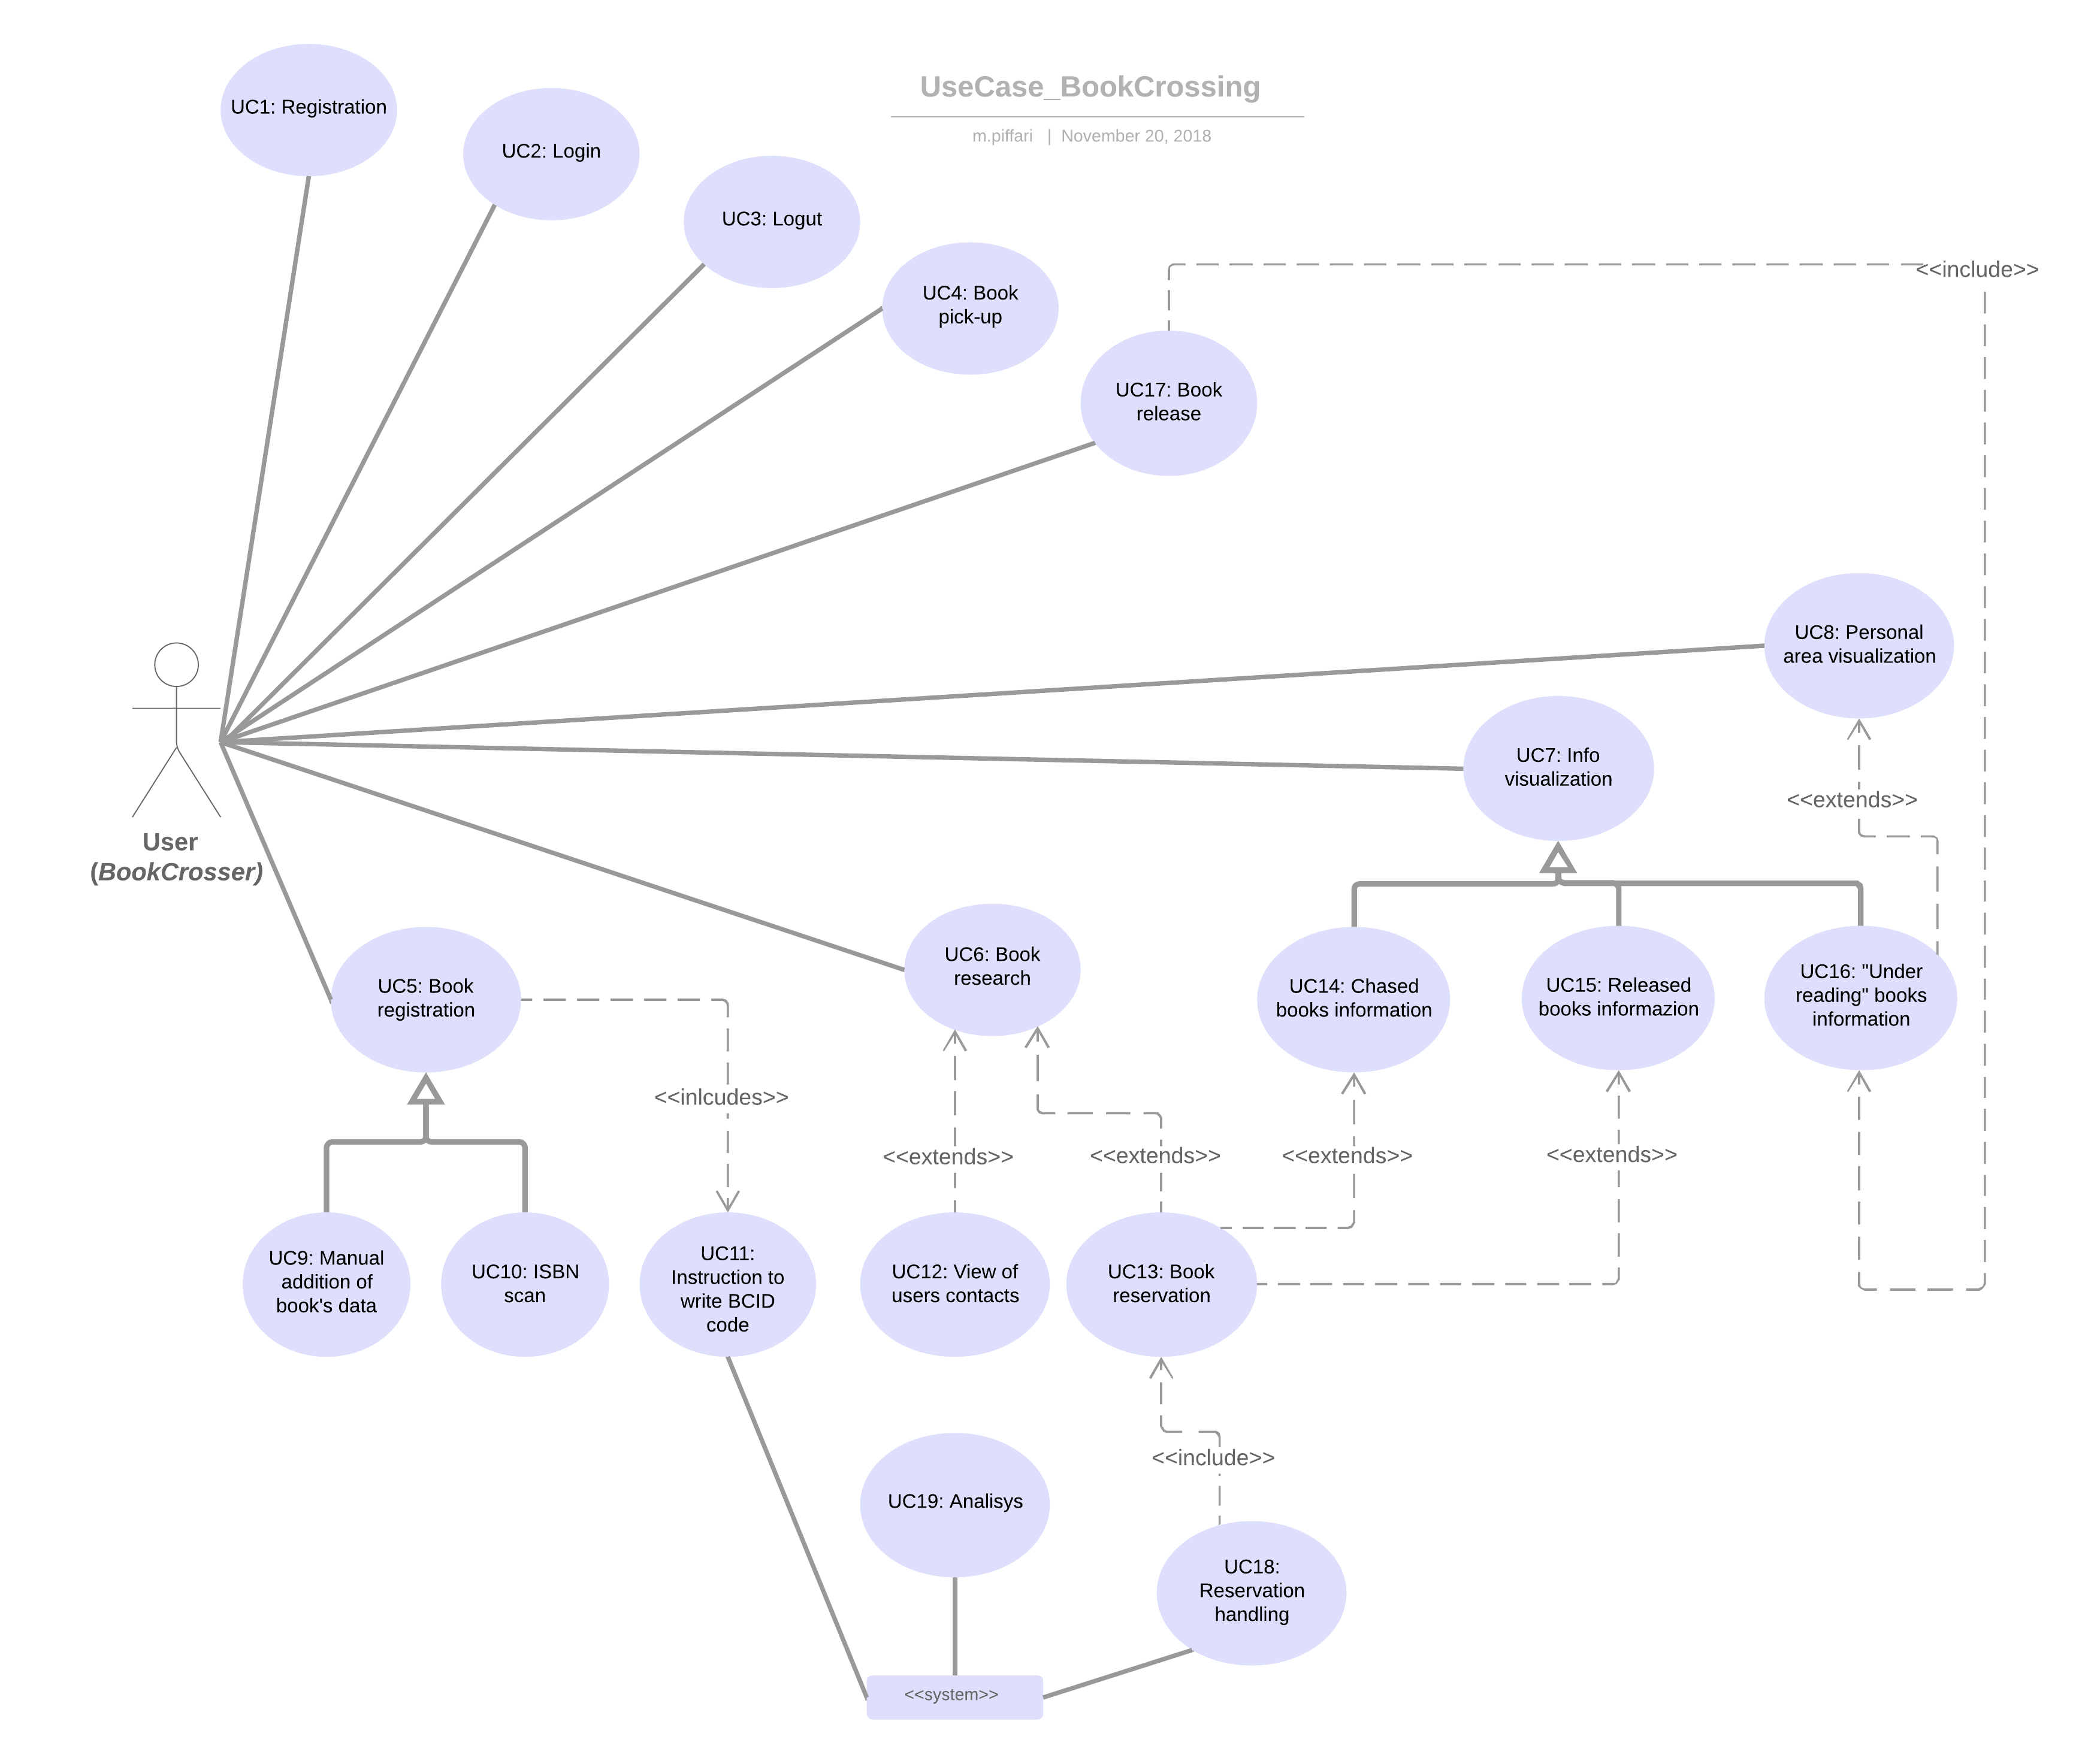
\includegraphics[width=\textwidth]{Immagini/UseCase_BookCrossing}
	\caption{Use cases diagram}
	\label{fig:UsecasesDiagram}
\end{figure}
\section{Funzionalità richieste}
\input{Capitolo_Sezioni/FunzionalitàRichieste}
\section{Specfiche del progetto bla bla bla}
\chapter{Architettura}
\section{Deployment diagram}
\begin{figure}[h]
	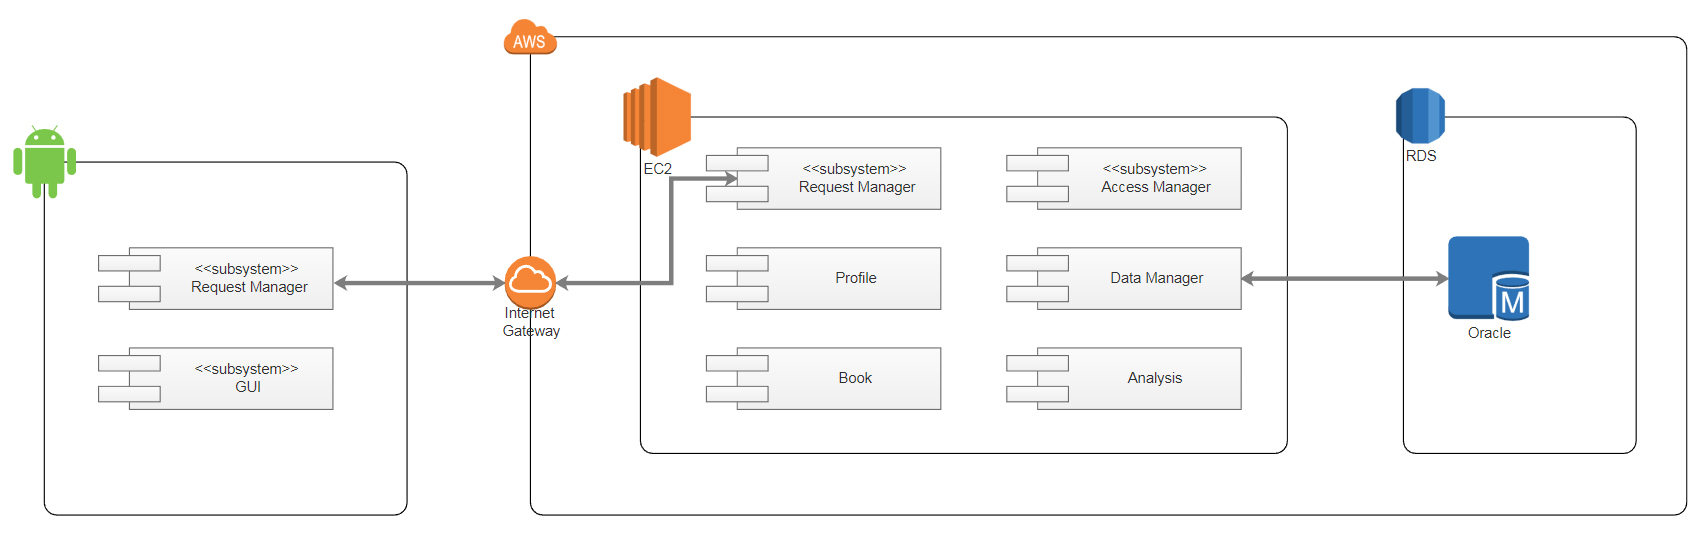
\includegraphics[width=\textwidth]{Immagini/Deployment_Diagram}
	\caption{Deployment Diagram}
	\label{fig:Deployment Diagram}
\end{figure}
\section{Architecture Envisioning}
\begin{figure}[h]
	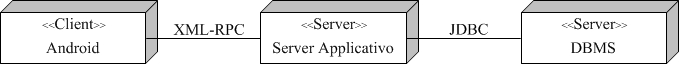
\includegraphics[width=\textwidth]{Immagini/Architecture_Envisoring}
	\caption{Architecture Envisoring}
	\label{fig:ArchitectureEnvisoring}
\end{figure}
\section{Architettura software}
\begin{figure}[h]
	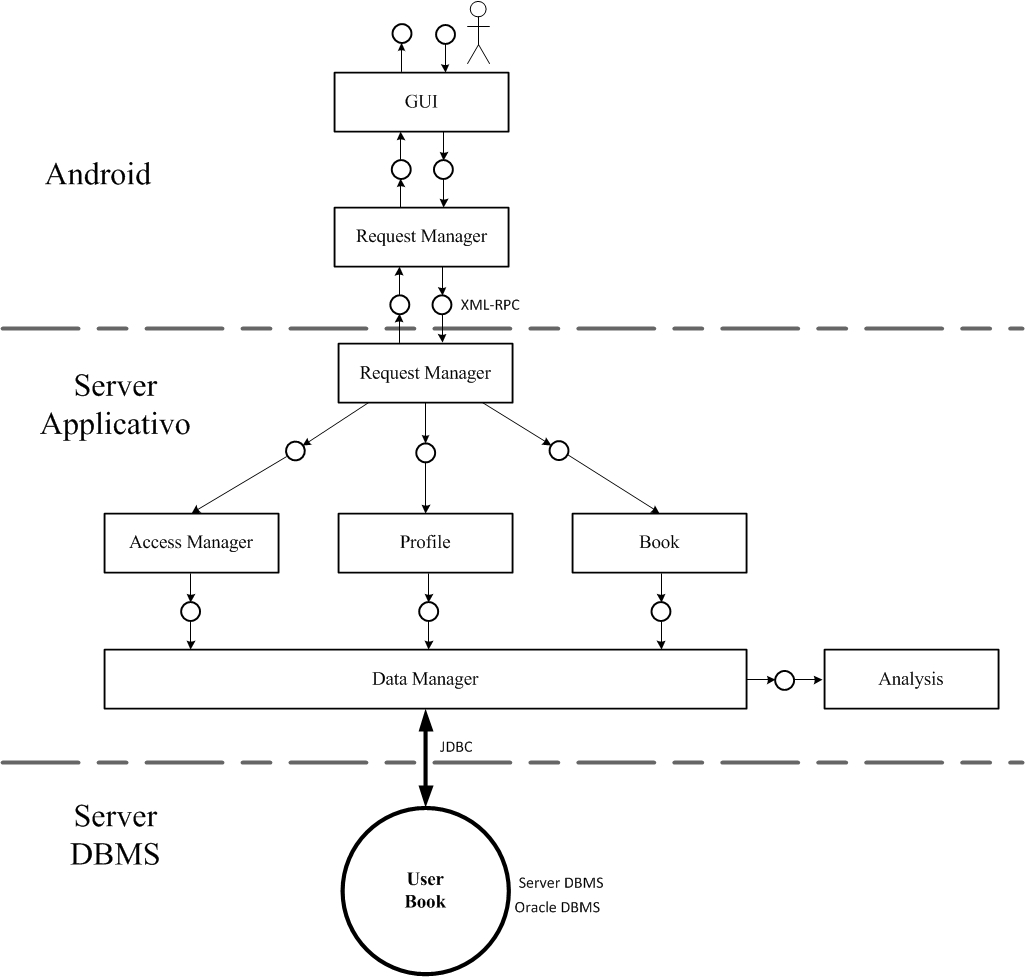
\includegraphics[width=\textwidth]{Immagini/Architettura_Software}
	\caption{Architettura Software}
	\label{fig:ArchitetturaSoftware}
\end{figure}

\end{document}
